\documentclass[12pt]{../SOP2}
\usepackage[english]{babel}
\usepackage{blindtext}
\usepackage{lipsum}

%\documentclass{article}

%\documentclass[12pt]{~/github/SOPs/SOP_Template/SOP}

\title{General Laboratory Safety Plan}

\date{8/1/2016}
\author{EA Students, Fall 2015}
\approved{Los Huertos}
\ReviseDate{\today}
\SOPno{01.v01}

\usepackage{Sweave}
\begin{document}
\Sconcordance{concordance:Laboratory_Safety_v01.tex:Laboratory_Safety_v01.Rnw:%
1 17 1 1 0 213 1}


\maketitle



\section{Scope and Application}

\NP The objective of lab safety manual is to create a safe operating space for students.

\NP This Laboratory Safety Plan is a draft and requires on-going updating, editting, and expansion as incidents occur and lessons learned. 


\section{Summary of Method}

\NP Researchers working the lab have been working since the fall of 2015 to develop this document from a range of resources. 

\NP Many of the contributions have been researched by students but require additional information, editting and professional insight.

\NP The \href{http://safetyservices.ucdavis.edu/sites/default/files/documents/LabSafetyPlan_Template.docx}{template} available on UC Davis' web site will be used to improve the document in the 2016-2017 school year.

\tableofcontents

\section{Acknowledgements}

\subsection*{Student Contributions}

\NP EA030-Fall 2015: Benjamin Schmidt, Kay Garlick-Ott, Marc Los Huertos, Grace Hruska, Juan Jaramillo, Thomas Kelleher, RaSia Khepra, Alexander Landau, Peter Mellinger, Emelia von Saltza, Alexandra Tchaoucheva, Ki'Amber Thompson, Malone Mischke.



\section{Definitions}

\section{Interferences}

\section{Health and Safety}

\NP 

\section{Personnel \& Training Responsibilities}

\subsection*{Lab Equipment Training}

\NP A researcher (student, staff person, or professor) is not permitted to use the lab equipment until he or she has been appropriately trained to use the equipment.

\NP The purpose of requiring all students to be properly trained is so that experiments and tests can be performed safely and effectively.  

\NP Training for all of the equipment will be provided before anyone is permitted to use it.  After being trained, students will sign a document that assures they understand exactly how the equipment works and how it will be used.

\NP Training, while limited to the SOP in question, is completely only after the Training Documentation Form has been completed.

\NP As research progresses, training information for the equipment we use will be added to this section, along with the documents that the researchers must be trained.

\section{Required Materials}

\NP PPE...



\section{Estimated Time}

\NP This will take XX minutes...

\section{Procedure}

\subsection*{General Emergency Response}

\NP The general emergency response procedures for earthquakes, fires and evacuations, medical emergencies, crimes, bomb threats, utility failures, and hazardous spills are described in the Pomona Emergency Brochure hanging in each laboratory (usually located near exits). You can also find the brochure online: \href{http://www.pomona.edu/sites/default/files/emergency-instructions.pdf}. Each individual within the lab is required to review the Emergency Brochure and certify that they have understand the information before starting a lab activity.

\NP Below is a brief summary of the most important information inside the Emergency Brochure: 

\begin{table}
\begin{tabular}{lll} \hline
Office            & Phone Number & Hours \\ \hline\hline
Campus Safety     & (909)607-2000 (from a campus phone, dial x72000) & Open 24/7 \\ \hline
\end{tabular}
\end{table}

\NP Upon answering be ready to provide the following information:

\begin{itemize}
  \item Your name
  \item Location of emergency
  \item Contact phone number(s)
\end{itemize}

\NP Campus Safety will assess the situation and call any necessary services (e.g. ambulance, fire department, etc.)

\NP Pomona College On-Call Deans and the Monsour On-Call Counselor are reachable via Campus Safety's emergency number. 

\NP For non-emergency numbers where information is needed, call 
 
\begin{itemize}
  \item CUC Student Health Services: 909-621-8222
  \item CUC Environmental Health \& Safety: 909-621-8538 
\end{itemize}

\NP Lab Contract list is posted in SGM 133. Please note it's location.

\subsection*{Earthquakes Procedure} 

\NP asfasdf

\begin{description}
  \item[Indoor Reponose] Move away from windows, filing cabinets, shelves, chemicals and other heavy objects which may fall. "Duck, Cover, and Hold" until shaking stops. If you are not near a table or sturdy desk, crouch against an interior wall or between seating rows in an auditoriums, and cover your neck and head. If you’re standing in a doorway, brace yourself against the frame, with your back to the door.

Once shaking stops, leave the building. Take any necessary items with you (e.g. phone, wallet, medication) and go to the nearest Pomona College evacuation site and wait for further instructions. If possible, put on shoes as there could be broken debris. 

DO NOT USE ELEVATORS!

\item[Outdoor Reponse] Move away from buildings, trees, signs, electrical poles and wires.
Protect your head and neck (in case of falling debris).
After shaking stops, go to the nearest Pomona College evacuation site and wait for further instructions (please see Campus Emergency Evacuation Sites map below).

\end{description}
	
	*AFTERSHOCKS MAY OCCUR.* Be Prepared!


\subsection*{Fires \& Evacuation Procedures}

Please see "Fires" below under "Lab Emergency Response"

\subsection{Medical Emergencies}

\NP Call Campus Safety. Let Campus Safety know the victim's condition. 

\NP Provide necessary first aid until Campus Safety and/or emergency services arrive.

\NP See Campus Emergency Evacuation Sites Map for AED locations (Figure \ref{fig:evacmap}).

\begin{figure}
\label{fig:evacmap}
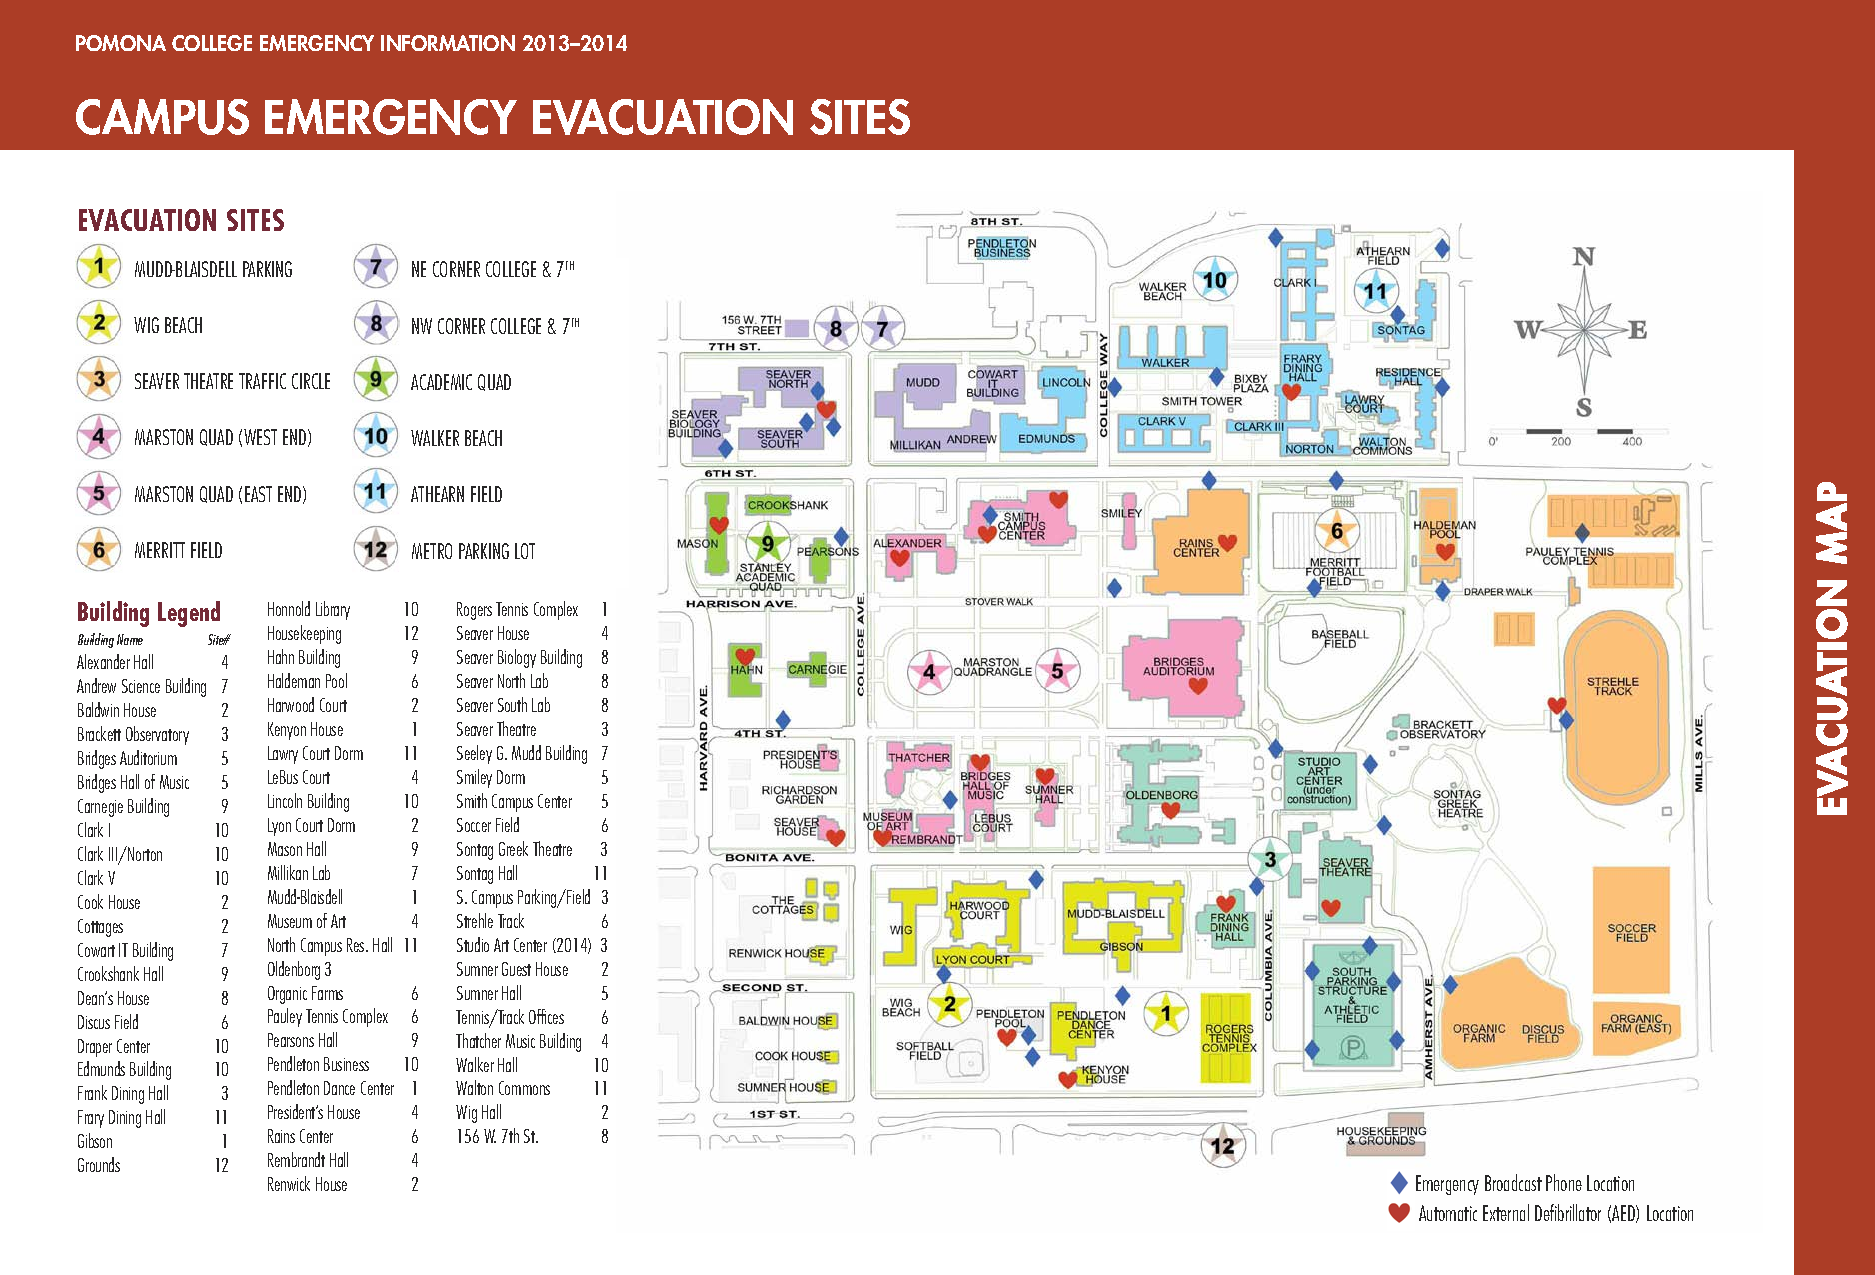
\includegraphics{evacuation-map.pdf}
\end{figure}

\subsection*{Crime on Campus}

\NP Report all crimes and suspicious activity on or near campus to Campus Safety.

\begin{description}
  \item[Active Shooter]If shooter is in a building, exit the building if it is safe to do so. Find a safe location. Call Campus Safety.
  \item[Campus Lockdown] If leaving a building is not possible or if a campus lockdown is enacted:
\begin{itemize}
  \item Go to the nearest room.
  \item Close and lock door (if there’s no lock, barricade the door with heavy objects).
  \item Turn off lights. Pull down window shades.
  \item Keep quiet. Silence phones.
  \item Call Campus Safety.
\end{itemize}
  \item[Bomb Threat \& Utilities Failure](please review the Emergency Brochure for more information)
\end{description}

\subsection{Hazardous Materials Spills}

\NP Refer to "Chemical Spills" in SOP02 Handling of Hazardous Materials"and the Emergency Brochure for detailed information on the procedures for Minor and Major Chemical Spills.

\subsection{Campus Emergency Evacuation Sites}

See Figure \ref{fig:evacmap} and (\href{Pomona College Emergiency Instruction}{http://www.pomona.edu/sites/default/files/emergency-instructions.pdf}

\subsection*{Emergency Procedures - Lab}

\NP At minimum these are the responses you should know. Look at the SDS (Safety Data Sheets) for more detailed instructions on how to respond for the particular chemicals.  

\NP In the case of a small fire, you may attempt to use a fire extinguisher to douse the flames (Make sure to know the location of the fire extinguisher within your laboratory). 
When dealing with a fire, remember:

\begin{itemize}
  \item Remove people from the area
  \item Activate the closest fire alarm
  \item Call Campus Safety
  \item Extinguish the fire, if safe
    \begin{enumerate}
      \item When using a fire extinguisher, place yourself between the fire and the exit; 
	    \item Pull the pin
	    \item Aim the nozzle towards the base of the fire
	    \item Squeeze the handle to release the extinguishing agent
	    \item Sweep the base of the fire from side to side
    \end{enumerate}

  \item Only use one fire extinguisher; if the fire cannot be put after after discharging one fire extinguisher, do not attempt to find another. Instead, leave the room, close the door behind you, and go to the nearest Pomona College evacuation site and wait for instructions.
  
\end{itemize}

\NP If trapped in a building:
\begin{itemize}
  \item Call Campus Safety
  \item Close all windows and doors\
  \item Wet and place cloth material around and under door to prevent smoke from entering
\end{itemize}

\NP If there is a hazardous chemical spill in the laboratory do not attempt to clean it up.  Appropriate attire and methods are required in order to prevent injury.  Contact lab instructor or supervisor for further instruction. If chemicals get in your eye, flush eye for 15 minutes at the eyewash station.  Additionally, if toxic materials are spilled on your body, remove all clothing and stand beneath the lab shower for 15 minutes. In the event of inhalation, move to fresh air, and find further information on the chemical inhaled.  

\NP If someone is at risk protect yourself first, only provide assistance if you can do so safely.  Alert your supervisor of the situation so that proper actions can be taken.

\section{References}

\NP \href{http://emergency.cdc.gov/disasters/earthquakes/prepared.asp}{Earthquake Preparedness}

\NP \href{http://safetyservices.ucdavis.edu/sites/default/files/documents/LabSafetyPlan_Template.docx}{UC Davis Lab Safety Template}

\NP \href{https://www.dartmouth.edu/~chemlab/info/safety/hazards.html}{Dartmouth College Safety Resources}

\NP \href{http://www.csb.gov/file.aspx?DocumentId=420}{TTU Lab Explosion Case Study}

\NP \href{https://sakai.claremont.edu/access/content/group/CX_mtg_87013/Project%201%3A%20Lab%20and%20Field%20Safety/Lessons%20Learned/Lesson_Learned_Report.pdf}{Pomona College Lessons Learned}

\NP \href{https://ehs.stonybrook.edu/programs/laboratory-safety}{Stony Brook Lab Safety Information}

\NP APHA, AWWA. WEF. (2012) Standard Methods for examination of water and wastewater. 22nd American Public Health Association (Eds.). Washington. 1360 pp. (2014).

\end{document}
